\documentclass{standalone}
\usepackage{tikz}
\usetikzlibrary{patterns, positioning}


\begin{document}
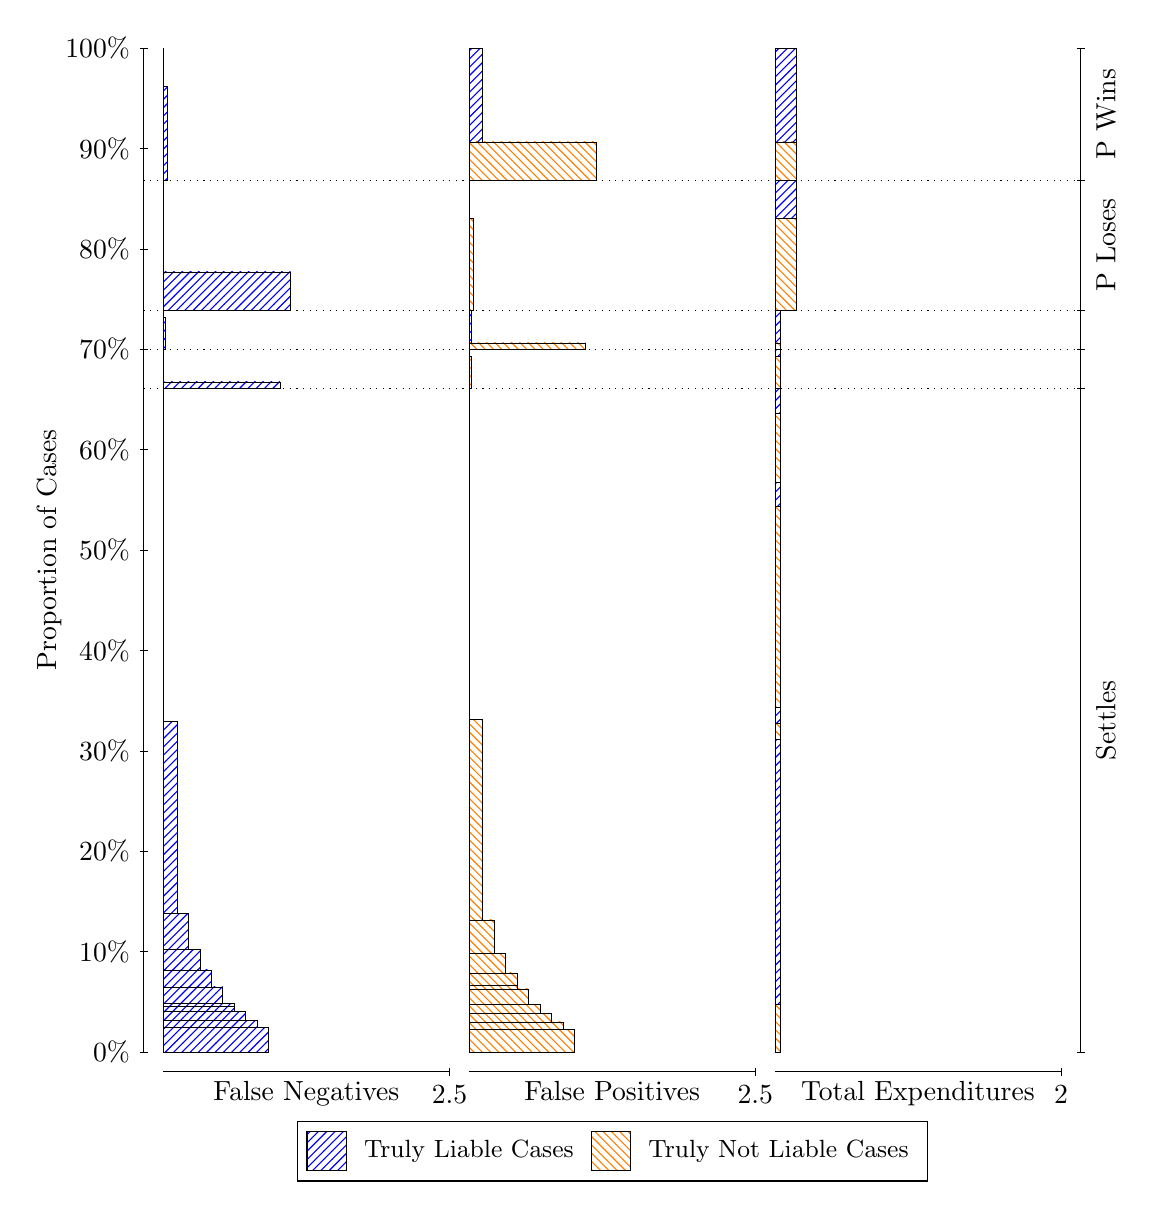
\begin{tikzpicture}
\draw[black, very thin] (1.5,1.75) -- (1.5,14.5);
\node[rotate=90, text=black, anchor=center] at (0.3, 8.125) {Proportion of Cases};
\draw[black, very thin] (1.45,1.75) -- (1.55,1.75);
\node[text=black, anchor=east] at (1.45, 1.75) {0\%};
\draw[black, very thin] (1.45,3.025) -- (1.55,3.025);
\node[text=black, anchor=east] at (1.45, 3.025) {10\%};
\draw[black, very thin] (1.45,4.3) -- (1.55,4.3);
\node[text=black, anchor=east] at (1.45, 4.3) {20\%};
\draw[black, very thin] (1.45,5.575) -- (1.55,5.575);
\node[text=black, anchor=east] at (1.45, 5.575) {30\%};
\draw[black, very thin] (1.45,6.85) -- (1.55,6.85);
\node[text=black, anchor=east] at (1.45, 6.85) {40\%};
\draw[black, very thin] (1.45,8.125) -- (1.55,8.125);
\node[text=black, anchor=east] at (1.45, 8.125) {50\%};
\draw[black, very thin] (1.45,9.4) -- (1.55,9.4);
\node[text=black, anchor=east] at (1.45, 9.4) {60\%};
\draw[black, very thin] (1.45,10.675) -- (1.55,10.675);
\node[text=black, anchor=east] at (1.45, 10.675) {70\%};
\draw[black, very thin] (1.45,11.95) -- (1.55,11.95);
\node[text=black, anchor=east] at (1.45, 11.95) {80\%};
\draw[black, very thin] (1.45,13.225) -- (1.55,13.225);
\node[text=black, anchor=east] at (1.45, 13.225) {90\%};
\draw[black, very thin] (1.45,14.5) -- (1.55,14.5);
\node[text=black, anchor=east] at (1.45, 14.5) {100\%};

\draw[black, very thin] (13.4,1.75) -- (13.4,14.5);
\draw[black, very thin] (13.35,1.75) -- (13.45,1.75);
\node[anchor=west] at (13.35, 1.75) {};
\draw[black, very thin] (13.35,10.177) -- (13.45,10.177);
\node[anchor=west] at (13.35, 10.177) {};
\draw[black, very thin] (13.35,10.674) -- (13.45,10.674);
\node[anchor=west] at (13.35, 10.674) {};
\draw[black, very thin] (13.35,11.169) -- (13.45,11.169);
\node[anchor=west] at (13.35, 11.169) {};
\draw[black, very thin] (13.35,12.821) -- (13.45,12.821);
\node[anchor=west] at (13.35, 12.821) {};
\draw[black, very thin] (13.35,14.5) -- (13.45,14.5);
\node[anchor=west] at (13.35, 14.5) {};

\draw[black, very thin, pattern color=blue, pattern=north east lines] (1.75,1.75) rectangle (3.0852,2.0582);
\draw[black, very thin, pattern color=blue, pattern=north east lines] (1.75,2.0582) rectangle (2.9399,2.1524);
\draw[black, very thin, pattern color=blue, pattern=north east lines] (1.75,2.1524) rectangle (2.7946,2.2672);
\draw[black, very thin, pattern color=blue, pattern=north east lines] (1.75,2.2672) rectangle (2.6492,2.3278);
\draw[black, very thin, pattern color=blue, pattern=north east lines] (1.75,2.3278) rectangle (2.6492,2.3713);
\draw[black, very thin, pattern color=blue, pattern=north east lines] (1.75,2.3713) rectangle (2.5039,2.5758);
\draw[black, very thin, pattern color=blue, pattern=north east lines] (1.75,2.5758) rectangle (2.3586,2.7926);
\draw[black, very thin, pattern color=blue, pattern=north east lines] (1.75,2.7926) rectangle (2.2133,3.0514);
\draw[black, very thin, pattern color=blue, pattern=north east lines] (1.75,3.0514) rectangle (2.0679,3.5096);
\draw[black, very thin, pattern color=blue, pattern=north east lines] (1.75,3.5096) rectangle (1.9226,5.949);
\draw[black, very thin, pattern color=orange, pattern=north west lines] (1.75,5.949) rectangle (1.75,10.177);
\draw[black, very thin, pattern color=blue, pattern=north east lines] (1.75,10.177) rectangle (3.2306,10.261);
\draw[black, very thin, pattern color=orange, pattern=north west lines] (1.75,10.261) rectangle (1.75,10.674);
\draw[black, very thin, pattern color=blue, pattern=north east lines] (1.75,10.674) rectangle (1.7773,11.086);
\draw[black, very thin, pattern color=orange, pattern=north west lines] (1.75,11.086) rectangle (1.75,11.169);
\draw[black, very thin, pattern color=blue, pattern=north east lines] (1.75,11.169) rectangle (3.3668,11.657);
\draw[black, very thin, pattern color=orange, pattern=north west lines] (1.75,11.657) rectangle (1.75,12.821);
\draw[black, very thin, pattern color=blue, pattern=north east lines] (1.75,12.821) rectangle (1.8045,14.012);
\draw[black, very thin, pattern color=orange, pattern=north west lines] (1.75,14.012) rectangle (1.75,14.5);
\draw[black, very thin, pattern color=orange, pattern=north west lines] (5.6333,1.75) rectangle (6.9686,2.0348);
\draw[black, very thin, pattern color=orange, pattern=north west lines] (5.6333,2.0348) rectangle (6.8233,2.1326);
\draw[black, very thin, pattern color=orange, pattern=north west lines] (5.6333,2.1326) rectangle (6.6779,2.245);
\draw[black, very thin, pattern color=orange, pattern=north west lines] (5.6333,2.245) rectangle (6.5326,2.3499);
\draw[black, very thin, pattern color=orange, pattern=north west lines] (5.6333,2.3499) rectangle (6.3873,2.5511);
\draw[black, very thin, pattern color=orange, pattern=north west lines] (5.6333,2.5511) rectangle (6.2419,2.5983);
\draw[black, very thin, pattern color=orange, pattern=north west lines] (5.6333,2.5983) rectangle (6.2419,2.7545);
\draw[black, very thin, pattern color=orange, pattern=north west lines] (5.6333,2.7545) rectangle (6.0966,3.0046);
\draw[black, very thin, pattern color=orange, pattern=north west lines] (5.6333,3.0046) rectangle (5.9513,3.4272);
\draw[black, very thin, pattern color=orange, pattern=north west lines] (5.6333,3.4272) rectangle (5.8059,5.9779);
\draw[black, very thin, pattern color=blue, pattern=north east lines] (5.6333,5.9779) rectangle (5.6333,10.177);
\draw[black, very thin, pattern color=orange, pattern=north west lines] (5.6333,10.177) rectangle (5.6606,10.59);
\draw[black, very thin, pattern color=blue, pattern=north east lines] (5.6333,10.59) rectangle (5.6333,10.674);
\draw[black, very thin, pattern color=orange, pattern=north west lines] (5.6333,10.674) rectangle (7.1139,10.756);
\draw[black, very thin, pattern color=blue, pattern=north east lines] (5.6333,10.756) rectangle (5.6606,11.169);
\draw[black, very thin, pattern color=orange, pattern=north west lines] (5.6333,11.169) rectangle (5.6878,12.333);
\draw[black, very thin, pattern color=blue, pattern=north east lines] (5.6333,12.333) rectangle (5.6333,12.821);
\draw[black, very thin, pattern color=orange, pattern=north west lines] (5.6333,12.821) rectangle (7.2502,13.309);
\draw[black, very thin, pattern color=blue, pattern=north east lines] (5.6333,13.309) rectangle (5.7968,14.5);
\draw[black, very thin, pattern color=orange, pattern=north west lines] (9.5167,1.75) rectangle (9.5848,2.3499);
\draw[black, very thin, pattern color=blue, pattern=north east lines] (9.5167,2.3499) rectangle (9.5848,5.723);
\draw[black, very thin, pattern color=orange, pattern=north west lines] (9.5167,5.723) rectangle (9.5848,5.9243);
\draw[black, very thin, pattern color=blue, pattern=north east lines] (9.5167,5.9243) rectangle (9.5848,6.1288);
\draw[black, very thin, pattern color=orange, pattern=north west lines] (9.5167,6.1288) rectangle (9.5848,8.6795);
\draw[black, very thin, pattern color=blue, pattern=north east lines] (9.5167,8.6795) rectangle (9.5848,8.9877);
\draw[black, very thin, pattern color=orange, pattern=north west lines] (9.5167,8.9877) rectangle (9.5848,9.8638);
\draw[black, very thin, pattern color=blue, pattern=north east lines] (9.5167,9.8638) rectangle (9.5848,10.177);
\draw[black, very thin, pattern color=orange, pattern=north west lines] (9.5167,10.177) rectangle (9.5848,10.59);
\draw[black, very thin, pattern color=blue, pattern=north east lines] (9.5167,10.59) rectangle (9.5848,10.674);
\draw[black, very thin, pattern color=orange, pattern=north west lines] (9.5167,10.674) rectangle (9.5848,10.756);
\draw[black, very thin, pattern color=blue, pattern=north east lines] (9.5167,10.756) rectangle (9.5848,11.169);
\draw[black, very thin, pattern color=orange, pattern=north west lines] (9.5167,11.169) rectangle (9.7892,12.333);
\draw[black, very thin, pattern color=blue, pattern=north east lines] (9.5167,12.333) rectangle (9.7892,12.821);
\draw[black, very thin, pattern color=orange, pattern=north west lines] (9.5167,12.821) rectangle (9.7892,13.309);
\draw[black, very thin, pattern color=blue, pattern=north east lines] (9.5167,13.309) rectangle (9.7892,14.5);
\draw[black, dotted] (1.5,10.177) -- (13.4,10.177);
\draw[black, dotted] (1.5,10.674) -- (13.4,10.674);
\draw[black, dotted] (1.5,11.169) -- (13.4,11.169);
\draw[black, dotted] (1.5,12.821) -- (13.4,12.821);
\draw[black, very thin] (1.75,1.5) -- (5.3833,1.5);
\node[text=black, anchor=north] at (3.5667, 1.5) {False Negatives};
\draw[black, very thin] (5.3833,1.45) -- (5.3833,1.55);
\node[text=black, anchor=north] at (5.3833, 1.45) {2.5};

\draw[black, very thin] (5.6333,1.5) -- (9.2667,1.5);
\node[text=black, anchor=north] at (7.45, 1.5) {False Positives};
\draw[black, very thin] (9.2667,1.45) -- (9.2667,1.55);
\node[text=black, anchor=north] at (9.2667, 1.45) {2.5};

\draw[black, very thin] (9.5167,1.5) -- (13.15,1.5);
\node[text=black, anchor=north] at (11.333, 1.5) {Total Expenditures};
\draw[black, very thin] (13.15,1.45) -- (13.15,1.55);
\node[text=black, anchor=north] at (13.15, 1.45) {2};

\node[text=black, centered, rotate=90] at (13.72, 5.9635) {Settles};


\node[text=black, centered, rotate=90] at (13.72, 11.995) {P Loses};
\node[text=black, centered, rotate=90] at (13.72, 13.66) {P Wins};

\draw (7.449999999999999,1.5) node[draw=none] (baseCoordinate) {};
\begin{scope}[align=center]
        \matrix[scale=0.5, draw=black, below=0.5cm of baseCoordinate, nodes={draw}, column sep=0.1cm]{
            \node[rectangle, draw, minimum width=0.5cm, minimum height=0.5cm, pattern color=blue, pattern=north east lines] {}; &
            \node[draw=none, font=\small, text=black] (B) {Truly Liable Cases}; &
            \node[rectangle, draw, minimum width=0.5cm, minimum height=0.5cm, pattern color=orange, pattern=north west lines] {}; &
            \node[draw=none, font=\small, text=black] (B) {Truly Not Liable Cases}; \\
            };
\end{scope}

\end{tikzpicture}
\end{document}